% Presentation 1 (10 min): build with  pdflatex P1.tex  (run from this directory; figures are in ../figures)
% Speaker notes are in \note{} blocks; to print a notes handout use \setbeameroption{show notes}.
\documentclass[aspectratio=169,11pt]{beamer}
\usepackage[T1]{fontenc}
\usepackage{lmodern,graphicx,booktabs,array,xcolor}
\graphicspath{{../figures/}}
\definecolor{navy}{HTML}{142B4D}\definecolor{accent}{HTML}{2A7DE1}\definecolor{amber}{HTML}{D98C2B}\definecolor{pale}{HTML}{EEF3FA}
\usetheme{default}\usefonttheme{professionalfonts}
\setbeamercolor{title}{fg=navy}\setbeamercolor{frametitle}{fg=navy}\setbeamercolor{normal text}{fg=black!85}
\setbeamerfont{frametitle}{series=\bfseries,size=\Large}
\setbeamertemplate{navigation symbols}{}
\setbeamertemplate{footline}{\hfill\scriptsize\color{black!55}CISC662 | Optimizing nanochat down to the assembly level\hspace{2em}\insertframenumber\hspace{1.5em}\vspace{0.5em}}
\setbeamertemplate{itemize item}{\color{accent}$\bullet$}
\newcommand{\key}[1]{\textcolor{navy}{\textbf{#1}}}
\newcommand{\stat}[3]{\begin{minipage}[c][2.2cm][c]{#1}\centering{\fontsize{26}{28}\selectfont\bfseries\color{#3}#2}\end{minipage}}
\title{Optimizing nanochat down to the assembly level}
\subtitle{NVPTX and AMDGCN: rewriting the hot GPU kernels of an LLM trainer, then reading their machine code}
\author{Talha Mahmood \and Hamza Mahmood}
\institute{CISC662 | Presentation 1}
\date{November 2026}
\begin{document}

\begin{frame}[plain]\titlepage
\note{HAMZA (30 s). Our project takes a small program that trains a language model, finds the slowest pieces that run on the GPU, rewrites them by hand, and reads the machine code the compiler produces, for NVIDIA and AMD. This is the first of two presentations: today is what we are doing and first results; December 17 is the final results.}
\end{frame}

\begin{frame}{What we are doing and why}
\begin{enumerate}
\item[\key{1}] \key{Pick the hot spots.} Profile one training step of nanochat; find which GPU operations cost the most time.
\item[\key{2}] \key{Rewrite them by hand.} Fused Triton kernels first, then CUDA and HIP versions of the three most important ones.
\item[\key{3}] \key{Read the machine code.} Compile for NVIDIA (PTX, SASS) and AMD (AMDGCN); explain every speedup or slowdown by the instructions.
\end{enumerate}
\vfill\small\color{black!60}Baselines to beat: eager PyTorch and \texttt{torch.compile} (Inductor), measured on the same GPU in the same job.
\note{HAMZA (1 min). nanochat is a small complete program that trains a GPT-style model on one GPU. Most of the time goes into a few kinds of GPU operations. PyTorch runs them one at a time (eager) or fuses them automatically (torch.compile). Our question: can hand-written kernels beat both, and what does the machine code tell us about why? We go down the whole stack: PyTorch, Triton, CUDA, HIP, then instructions: PTX and SASS for NVIDIA, AMDGCN for AMD.}
\end{frame}

\begin{frame}{Proposal versus reality: what changed and why}
\small\renewcommand{\arraystretch}{1.5}
\begin{tabular}{@{}p{2.3cm}p{2.9cm}p{5.6cm}p{2.7cm}@{}}
\toprule \key{} & \key{Proposal} & \key{What we do now} & \key{Status}\\ \midrule
Main GPU & DARWIN V100 & DeltaAI GH200 (H100-class) & Measured\\
AMD GPUs & MI100 / MI250X & AMDGCN compiled for gfx908, gfx90a, gfx942 & Static done\\
AMD measured & same & NCSA Delta MI100 / MI210 (access confirmed) & Node in maintenance\\
CPU reference & x86 EPYC & Grace (aarch64) CPU, raw and normalised & Planned\\
V100 / A100 & primary / extra & Static comparison of sm\_70, sm\_80, sm\_90a SASS & Planned\\ \bottomrule
\end{tabular}
\note{HAMZA (1 min). The proposal named a V100 cluster as main GPU. We cannot reach it from our allocation, so we use DeltaAI at NCSA: one GH200, an H100-class GPU. DeltaAI has no AMD GPUs, so we already compile our kernels for three AMD chips and analyse the instructions without running them (static). Last week we confirmed access to NCSA Delta, which has MI100 and MI210 GPUs. That node is in maintenance right now, so measured AMD numbers are for the second presentation. If asked why not DARWIN: we dropped it; everything is on NCSA systems now.}
\end{frame}

\begin{frame}{Method: a ladder from PyTorch down to instructions}
\centering
\begin{tabular}{@{}*{6}{>{\centering\arraybackslash}p{1.85cm}}@{}}
\colorbox{accent}{\parbox[c][1.5cm][c]{1.75cm}{\centering\color{white}\textbf{L0}\\Eager}} &
\colorbox{accent}{\parbox[c][1.5cm][c]{1.75cm}{\centering\color{white}\textbf{L1}\\compile}} &
\colorbox{accent}{\parbox[c][1.5cm][c]{1.75cm}{\centering\color{white}\textbf{L2}\\Triton}} &
\colorbox{pale}{\parbox[c][1.5cm][c]{1.75cm}{\centering\color{navy}\textbf{L3}\\CUDA}} &
\colorbox{pale}{\parbox[c][1.5cm][c]{1.75cm}{\centering\color{navy}\textbf{L4}\\HIP (AMD)}} &
\colorbox{pale}{\parbox[c][1.5cm][c]{1.75cm}{\centering\color{navy}\textbf{L5}\\PTX / SASS / AMDGCN}}
\end{tabular}

{\footnotesize\color{black!60}Filled = done for our three kernels. NVIDIA and static AMD instructions (L5) already read for them; CUDA and HIP (L3, L4) start next.}
\bigskip

\begin{columns}[T]
\column{0.32\textwidth}\colorbox{pale}{\parbox{0.95\linewidth}{\small\key{Correctness gate}\\ value and gradient checked against a 64-bit reference; no worse than PyTorch's own error}}
\column{0.32\textwidth}\colorbox{pale}{\parbox{0.95\linewidth}{\small\key{Timing rules}\\ GPU events, L2 cache flushed, 3 separate processes, bootstrap confidence intervals}}
\column{0.32\textwidth}\colorbox{pale}{\parbox{0.95\linewidth}{\small\key{Fair comparison}\\ baselines run in the same job on the same GPU; only gated rows are plotted}}
\end{columns}
\note{(1 min). The method is a ladder. L0 eager PyTorch. L1 torch.compile. L2 our Triton kernel. L3 CUDA. L4 HIP, the AMD version of CUDA. L5 reading the instructions. Every kernel must pass a correctness gate against a 64-bit reference before we may time it; every timing uses GPU events, flushes the cache, and repeats in three separate processes with confidence intervals. Three kernels are on the ladder: RMSNorm, QK-norm with RoPE, softcap with cross-entropy.}
\end{frame}

\begin{frame}{Baseline: compile already halves the step; the loss and norms are what remains}
\begin{columns}[c]
\column{0.64\textwidth}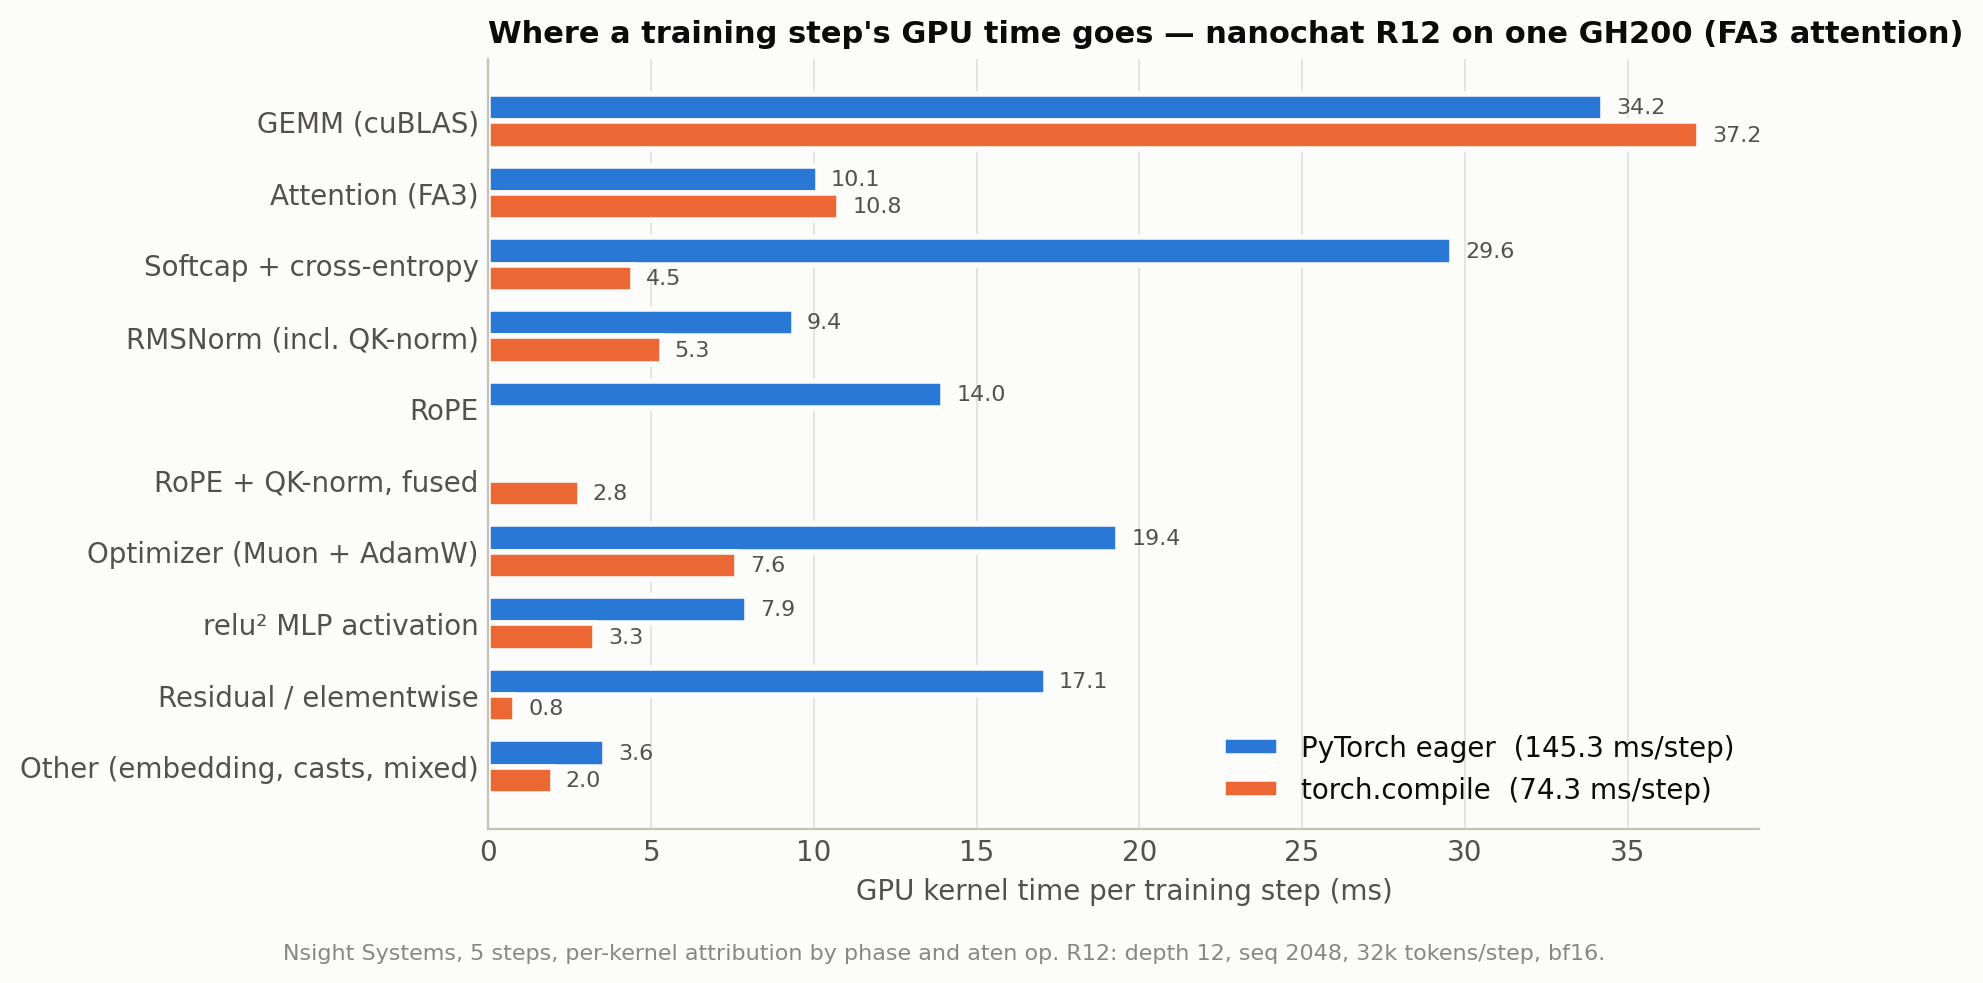
\includegraphics[width=\linewidth]{s1_kernel_breakdown.png}
\column{0.34\textwidth}\centering
\stat{\linewidth}{8.05 s}{accent}\\{\scriptsize per 100 steps, compile + FA3 (stock)}\\[4pt]
\stat{\linewidth}{15.08 s}{black!60}\\{\scriptsize per 100 steps, eager + FA3}\\[4pt]
\stat{\linewidth}{37\%}{amber}\\{\scriptsize model FLOP utilisation, compiled}
\end{columns}
\note{(1.3 min). Baseline to beat: 12-layer model, one GPU, bf16. Stock nanochat with torch.compile and FlashAttention-3 takes 8.05 s per 100 steps; eager takes 15.08 s, so compile already gives about 1.9 times. Matrix multiplications and attention dominate and use vendor libraries; we do not try to beat them. What is left is memory-bound operations: normalization, RoPE, the loss. The loss (softcap plus cross-entropy) is the largest one in eager at 29.6 ms; compile cuts it to 4.5 ms. Those are our targets.}
\end{frame}

\begin{frame}{First results: up to 2x over torch.compile and 12x over eager, with an honest tie}
\begin{columns}[c]
\column{0.62\textwidth}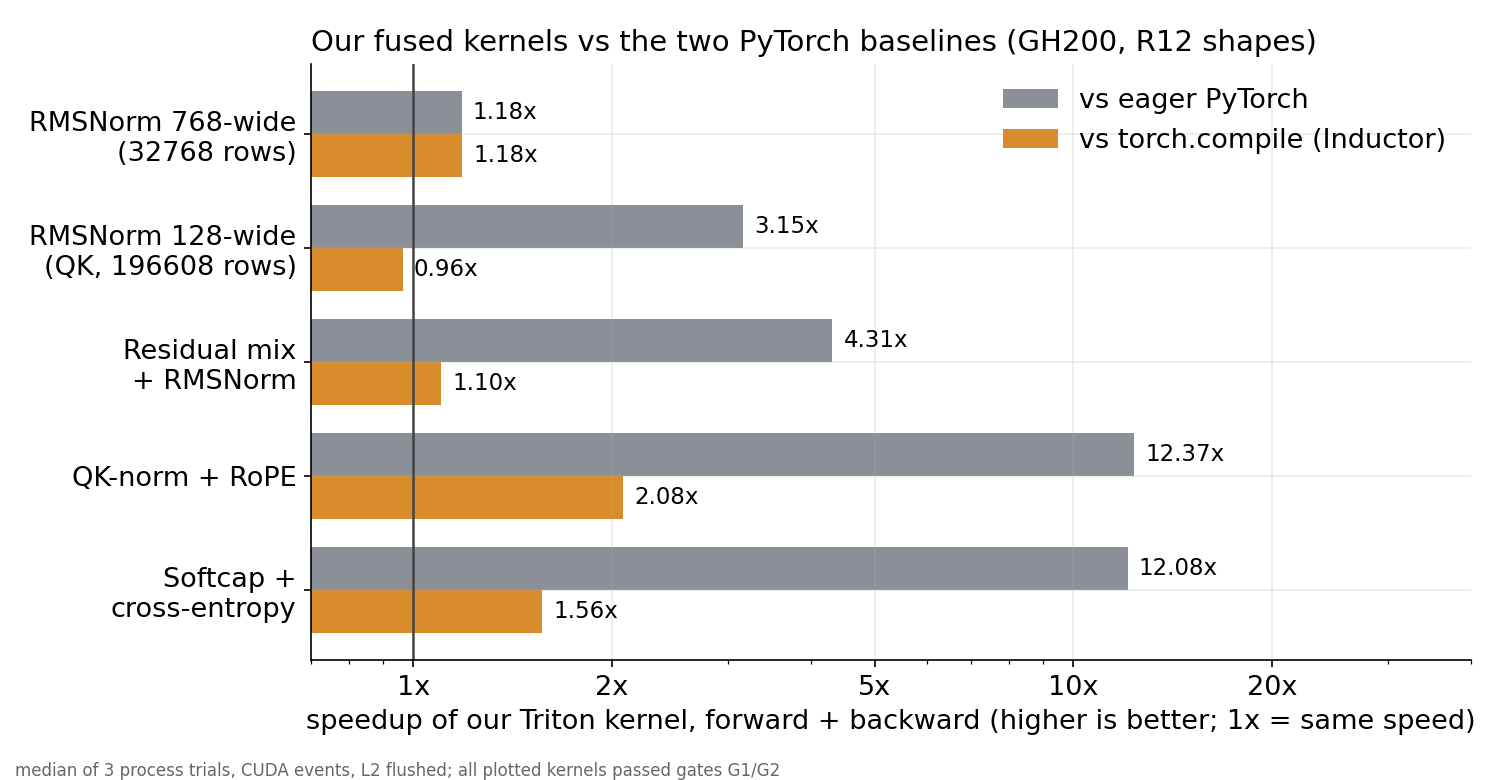
\includegraphics[width=\linewidth]{p1_kernel_speedups.png}
\column{0.36\textwidth}\small
\begin{itemize}
\item \key{Loss kernel:} 1.56x vs compile, 12.1x vs eager, 8x less memory (2.15 vs 17.2 GB)
\item \key{QK-norm + RoPE:} 2.08x vs compile
\item \key{RMSNorm:} 1.18x at 768 wide; a tie (0.96x) at 128 wide
\item {\color{black!60}All plotted kernels passed the correctness gates.}
\end{itemize}
\end{columns}
\note{(1.7 min). All measured on the GH200, forward plus backward. Grey is speedup over eager, orange over torch.compile, the harder baseline. The loss kernel is 12 times faster than eager, 1.56 over compile, and uses 8 times less memory. QK-norm plus RoPE is 12 over eager and 2 over compile. Residual-mix plus norm is 4.3 over eager and 1.1 over compile. Two honest points: for plain RMSNorm compile is already good, so only 1.18 times at 768 wide, and at 128 wide we tie compile (0.96, within noise). A result that is not better is still a result.}
\end{frame}

\begin{frame}{The machine code explains it: the loss kernel is limited by exp units, not memory}
\begin{columns}[c]
\column{0.52\textwidth}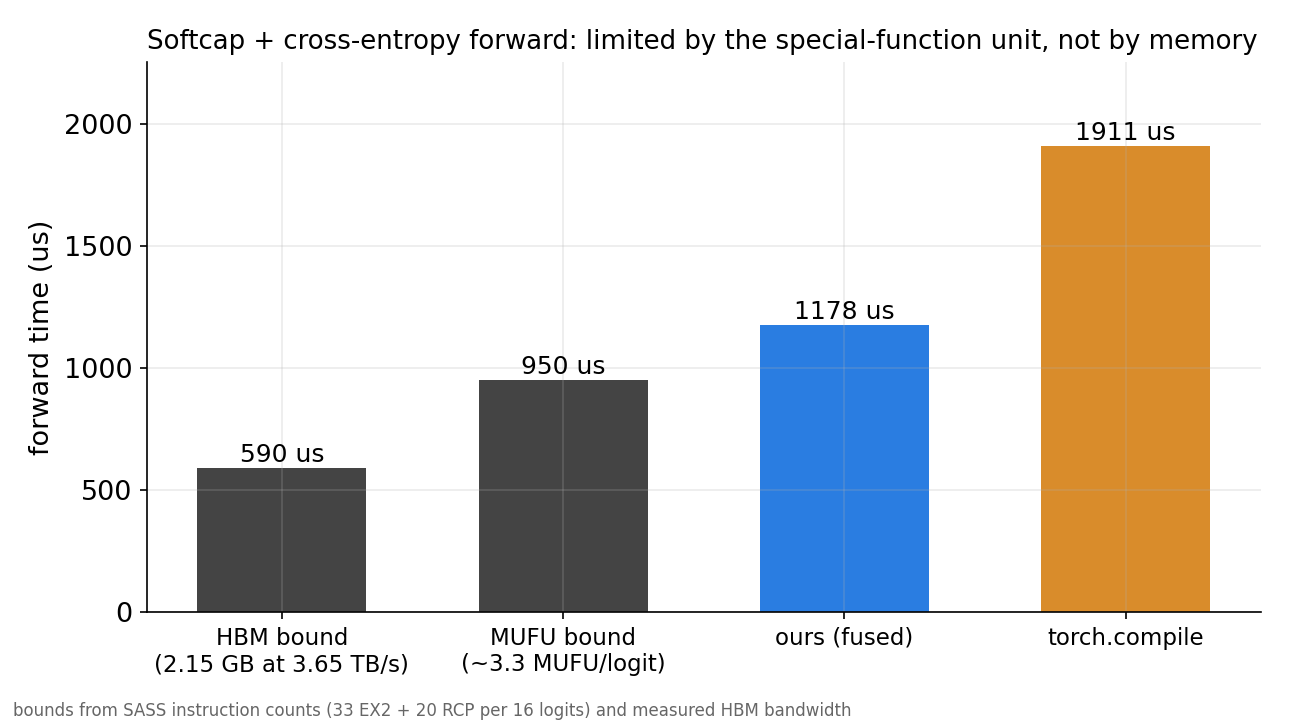
\includegraphics[width=\linewidth]{p1_ce_bounds.png}
\column{0.47\textwidth}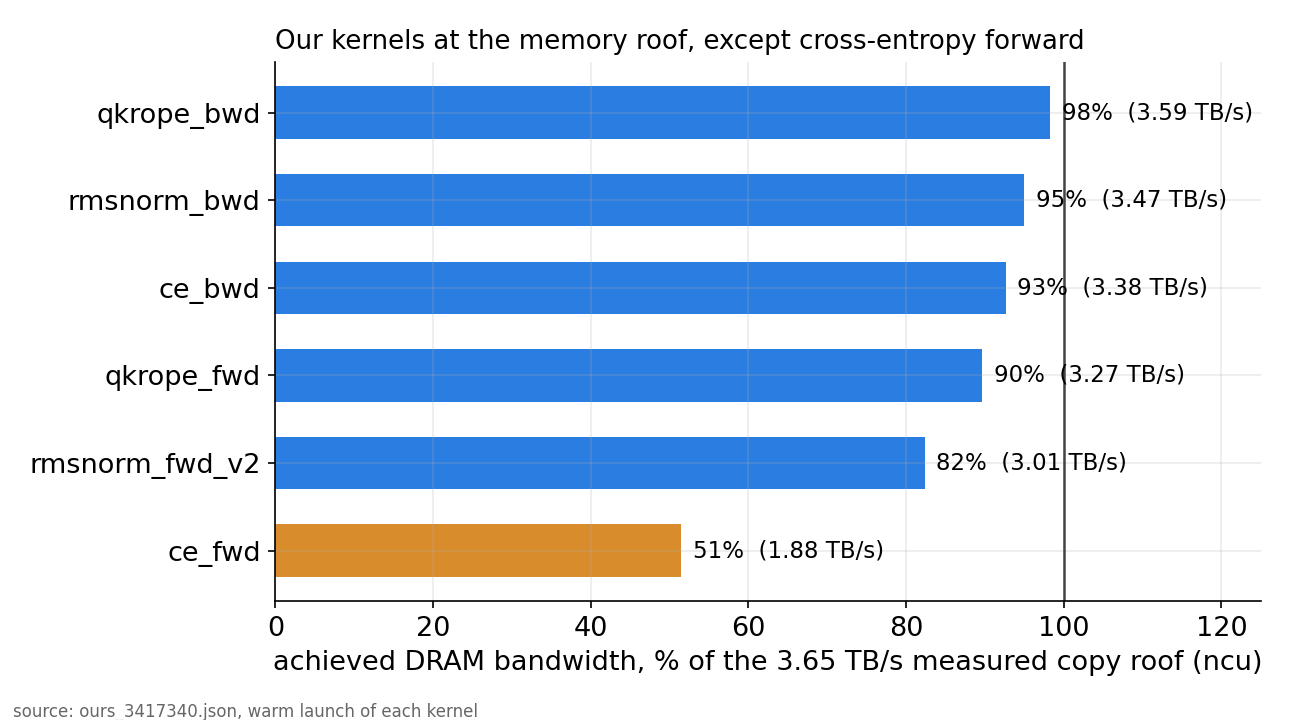
\includegraphics[width=\linewidth]{p1_bandwidth.png}
\end{columns}
\small\key{Evidence:} SASS has 33 EX2 + 20 RCP per 16 logits (about 3.3 special-function ops per logit). Compute floor 0.95 ms $>$ memory floor 0.59 ms; measured 1.18 ms. Other kernels sit at 82--98\% of the 3.65 TB/s measured bandwidth (Nsight Compute).
\note{(1.5 min). Our loss kernel moves little data, so we expected it to be memory-limited. The instruction analysis says otherwise: each logit needs about 3.3 operations on the special-function unit, the hardware that computes exp and reciprocal, and there are few of those units. That gives a floor of about 0.95 ms, above the 0.59 ms memory floor. We measure 1.18 ms, close to it. So the next improvement is fewer or cheaper exp instructions, not memory. A variant using the hardware's approximate tanh is faster still, but it is only an experiment, not adopted. Our other kernels run at 82 to 98 percent of measured bandwidth, so they are at the roof.}
\end{frame}

\begin{frame}{Plan to December 17, and the one real risk}
\begin{columns}[T]
\column{0.58\textwidth}\small
\begin{description}
\item[Now to Nov 20] Chunked loss + output layer, Triton GEMM and attention study, CUDA RMSNorm / RoPE
\item[Nov 20 to Dec 8] HIP ports, AMD tables, measured MI100/MI210 runs, plug into training and check the loss curve
\item[Dec 8] Code freeze, then final measurements
\item[Dec 17] Presentation 2: results
\end{description}
\column{0.38\textwidth}
\colorbox{pale}{\parbox{0.95\linewidth}{\small\key{Budget}\\ about 0.85 of 25 planned service units (SU) used}}\\[6pt]
\colorbox{pale}{\parbox{0.95\linewidth}{\small\key{Main risk}\\ AMD node in maintenance. Fallback: static AMDGCN analysis, already built.}}
\end{columns}
\note{HAMZA (1.3 min). Next month: the fused loss with the output layer so the huge logits tensor is never stored, a Triton matrix-multiplication study, an attention kernel, and CUDA and HIP versions of the three main kernels. In parallel the AMD side: static tables for all kernels, and measured runs on Delta once the node is back. Then plug the kernels into nanochat training and check the loss curve is unchanged, which is the gate that matters. Code freeze December 8; second presentation December 17. We have used about 0.85 of 25 planned SU, so cost is not the constraint. The main risk is AMD hardware availability; the fallback is the static analysis, already built.}
\end{frame}

\appendix
\begin{frame}{Backup: terms}
\small\renewcommand{\arraystretch}{1.4}
\begin{tabular}{@{}p{3.2cm}p{9cm}@{}}
\key{MUFU} & special-function unit: exp, reciprocal, tanh hardware\\
\key{ISA / SASS / PTX} & machine code; SASS is NVIDIA's real code, PTX the portable layer\\
\key{AMDGCN} & AMD's machine code; 64-thread wavefronts, MFMA matrix instructions\\
\key{Roofline} & chart of achieved speed against the memory and compute limits\\
\key{Gates G1 / G2} & value and gradient correctness against a 64-bit reference\\
\key{R12} & the test setup: 12 layers, sequence 2048, 32k tokens per step, bf16\\
\end{tabular}
\note{BACKUP. Use only for questions. A wavefront is AMD's 64-thread group; a warp is NVIDIA's 32.}
\end{frame}
\end{document}
